\documentclass[a4paper, 11pt]{article} % Font size (can be 10pt, 11pt or 12pt) and paper size (remove a4paper for US letter paper)

\usepackage[protrusion=true,expansion=true]{microtype} % Better typography
\usepackage{graphicx} % Required for including pictures
\usepackage{hyperref}
\usepackage{float}

\usepackage{mathpazo} % Use the Palatino font
\usepackage[T1]{fontenc} % Required for accented characters
\linespread{1.05} % Change line spacing here, Palatino benefits from a slight increase by default

\makeatletter
\renewcommand\@biblabel[1]{\textbf{#1.}} % Change the square brackets for each bibliography item from '[1]' to '1.'
\renewcommand{\@listI}{\itemsep=0pt} % Reduce the space between items in the itemize and enumerate environments and the bibliography

\renewcommand{\maketitle}{ % Customize the title - do not edit title and author name here, see the TITLE block below
\begin{flushright} % Right align
{\LARGE\@title} % Increase the font size of the title

\vspace{50pt} % Some vertical space between the title and author name

{\large\@author} % Author name
\\\@date % Date

\vspace{40pt} % Some vertical space between the author block and abstract
\end{flushright}
}

%----------------------------------------------------------------------------------------
%	TITLE
%----------------------------------------------------------------------------------------

\title{\textbf{Phylogeotool}\\ % Title
Reference Manual} % Subtitle

\author{\textsc{Ewout Vanden Eynden, Pieter Libin, Kristof Theys, anderen, Guy Baele} % Author
\\{\textit{Rega Institute}}} % Institution

\date{2016} % Date

%----------------------------------------------------------------------------------------

\begin{document}
\maketitle % Print the title section

\vspace{30pt} % Some vertical space between the abstract and first section

%------------------------------------------------
\tableofcontents
\newpage

\section{Installation}
\subsection{Preparations before installation}
\subsubsection*{Java}
Download and install the newest Java Development Kit (JDK) from \url{http://www.oracle.com/technetwork/java/javase/downloads/index.html}.
The current version of the tool was build on JDK 1.8.0\_31.
\subsubsection*{Tomcat}
Download and install the newest Tomcat version from \url{http://tomcat.apache.org}.
\subsubsection*{Github}
Download the code from \url{https://github.com/rega-cev/phylogeotool/}. The project is currently still private. During the trial period you can send an email to \href{mailto:ewout.vandeneynden@kuleuven.be}  {ewout.vandeneynden@kuleuven.be} with your Github account name to get read rights on the project.
\subsubsection*{Ant}
Download and install the newest Ant version from \url{http://ant.apache.org/} as we will use it to build our project.
The current version of the tool was build with Ant 1.9.4
%------------------------------------------------

\section{Data preparation}
After building the code, different jar files can be found in the dist folder. Their function is explained here.
\subsection{DistanceMatrix.jar}
Tool to create a distance matrix based on the phylogenetic tree that will be used in the PhyloGeoTool.
\\
DistanceMatrix.jar takes the following input values:
\begin{itemize}
\item phylo.tree: Link to the phylogenetic tree to be used in the PhyloGeoTool.
\item distance matrix: Link to the location where the distance matrix can be written.
\end{itemize}

\subsection{PreRender.jar}
Before any data can be shown to the user, a lot of calculations are done backend. To speed up the process, most of those calculations can be done beforehand.
\\
PreRender.jar is a multithreaded application meaning that it performs best on any Java version > 7. Lower Java versions do not support our implementation of multithreading and will thus fail.
\\
PreRender.jar takes the input files:
\begin{itemize}
\item phylo.tree: Link to the phylogenetic tree used in the PhyloGeoTool.
\item csvFile: Link to the csv file that connects nodes in the tool to attributes. Note: The id in the csv file has to be the same as the id of the nodes in the tree.
\item distance matrix: Link to the distance matrix that was generated from this tree.
\item folder xml tree: Link to the folder where this jar can write its resulting tree files.
\item folder xml clusters: Link to the folder where this jar can write its resulting cluster files.
\item folder xml csv: Link to the folder where this jar can write its resulting csv files.
\item folder figtree: Link to the folder where this jar can write its resulting figtree representations.
\end{itemize}

%------------------------------------------------
\section{Tool functionality}
\subsection{Basic functionality}

\begin{figure}[H]
\centering
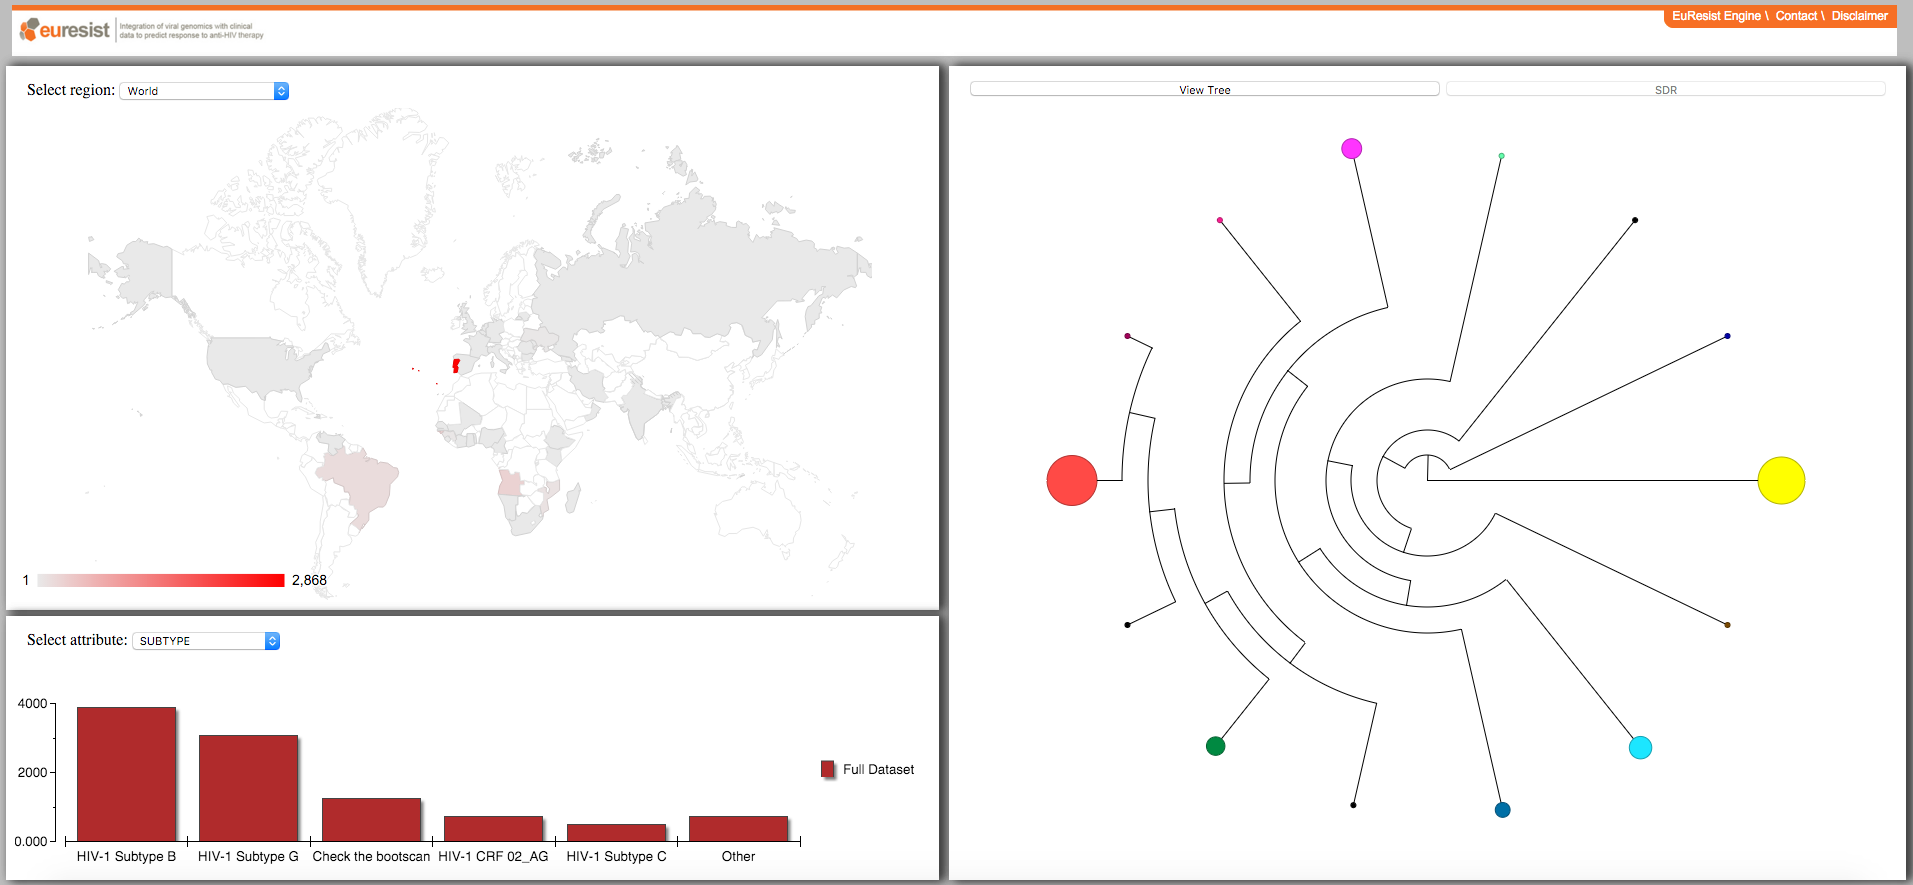
\includegraphics[width=400pt, height=400pt, keepaspectratio=true]{images/initial_view.PNG}
\caption{Initial view of the tool}
\label{fig:initial_view}
\end{figure}

The tool is divided into different area's
\begin{itemize}
  \item Top left shows a world map where each country is colored darker as more sequences are originating from here. It also contains a drop down box where you can select the region on which you want to zoom in (e.g. Europe, North-America, \ldots).
  \item Bottom left shows a bar chart which shows a certain attribute/characteristic from all sequences currently shown in the circular tree on the right. It also contains a drop down box where you can select the attribute/characteristic that you want to display in the bar chart. The attributes available for representation depend on the attributes given in the csv file.
  \item On the right, initially, the best clustering of the phylogenetic tree is shown. It also contains a button to visualise the tree in FigTree format.
\end{itemize}

\subsubsection{Hover over node in clustered tree}
\begin{figure}[H]
\centering
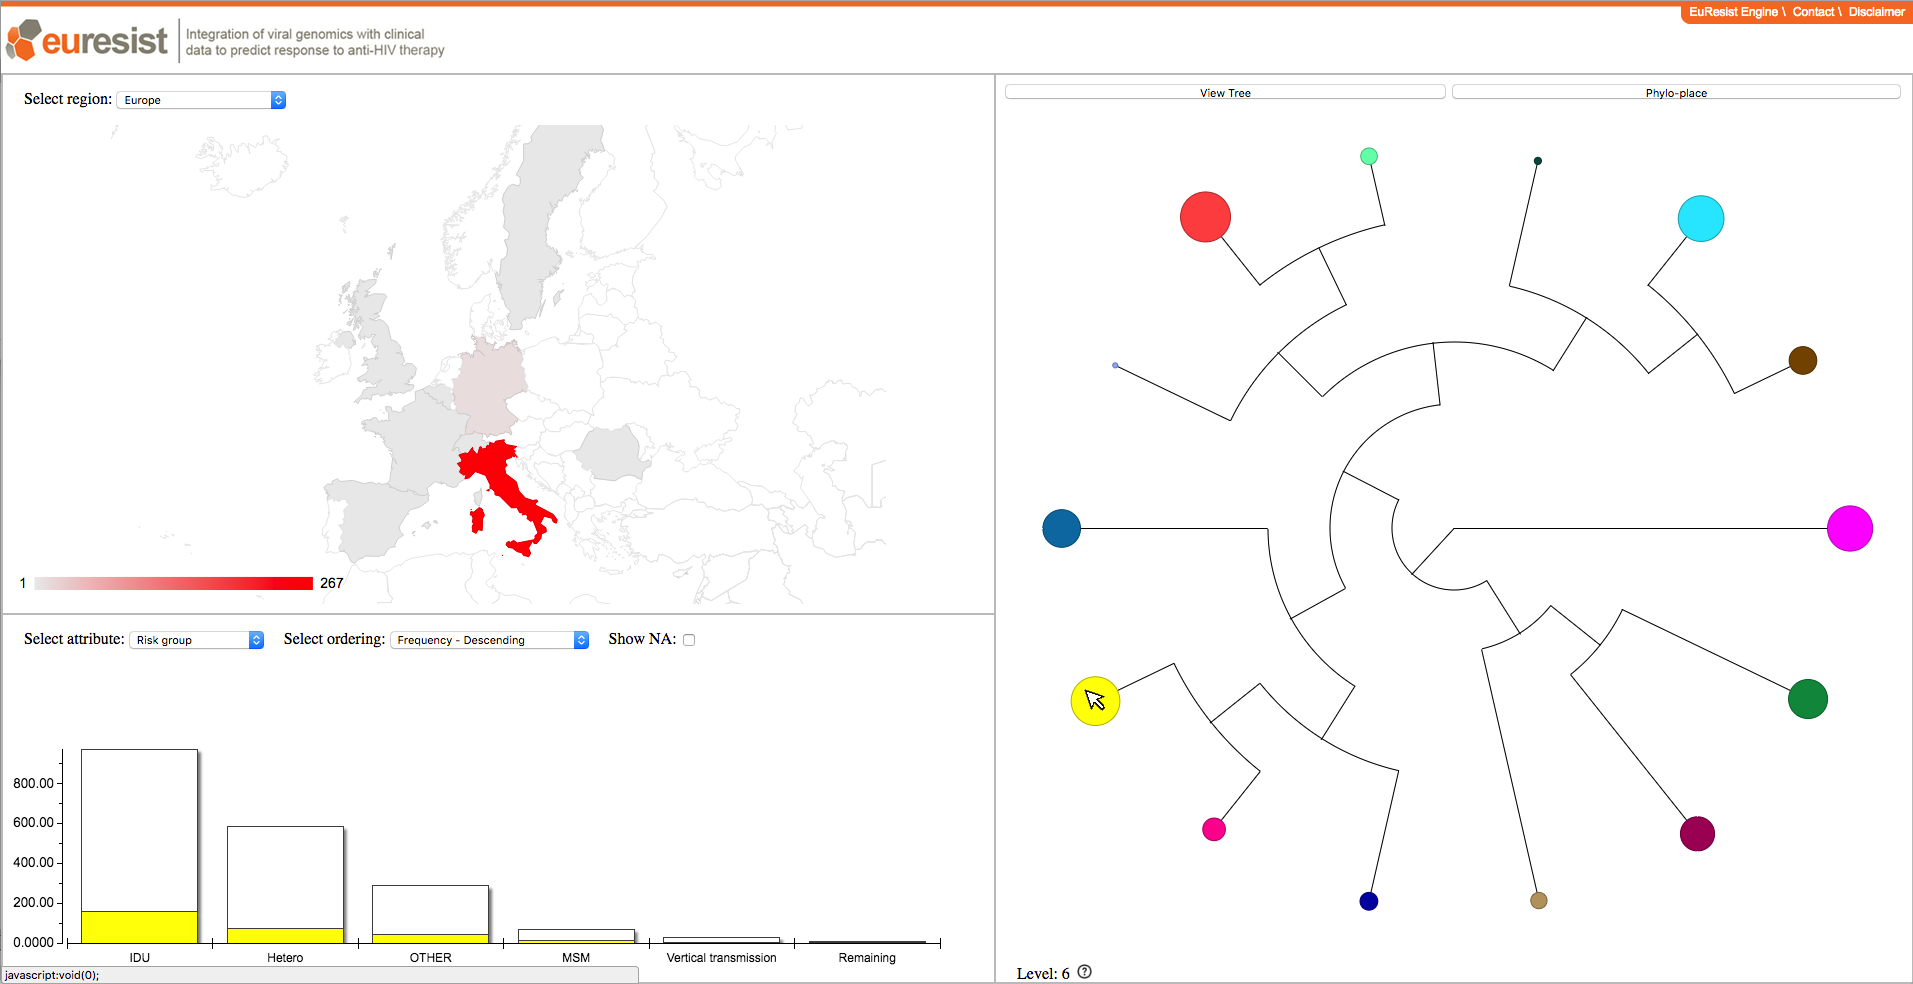
\includegraphics[width=400pt, height=400pt, keepaspectratio=true]{images/hover_node.PNG}
\caption{Hovering over a node in the tree}
\label{fig:hover_node}
\end{figure}

When you hover over a node in the phylogenetic tree, the bar chart on the bottom left and the map on the top left will be updated with data coming specifically from the node you hovered over.
\\
In the bar chart it'll be shown as an extra column that is added next to the already visible column.
\\
On the map it'll be shown as a new country colouring where each country is coloured based on only information coming from the hovered node.

\subsubsection{Change region}
\begin{figure}[H]
\centering
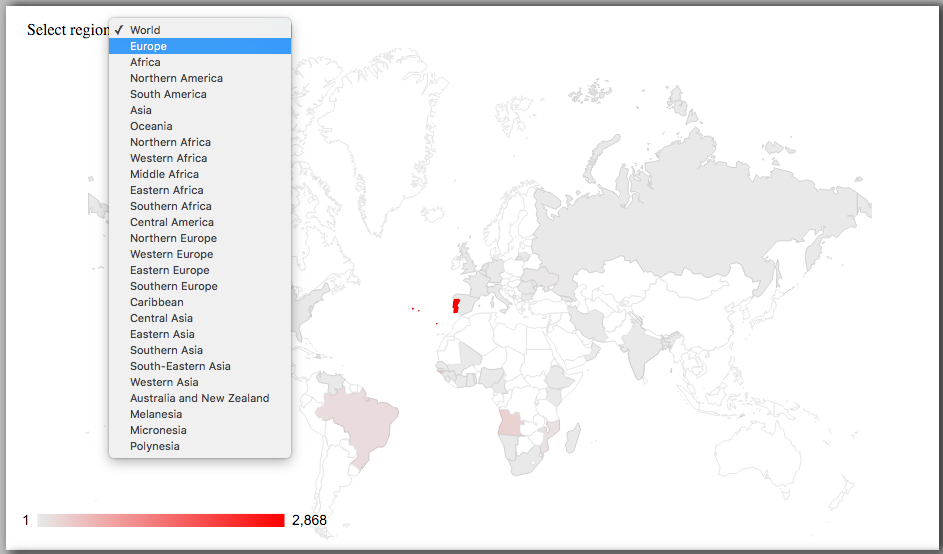
\includegraphics[width=400pt, height=400pt, keepaspectratio=true]{images/change_country.PNG}
\caption{Change the region in the drop down box}
\label{fig:change_region}
\end{figure}
When you change the region by selecting a new value in the drop down box on top of the map (see fig. \ref{fig:change_region}), the world map will update and now only show information originating from this specific region.

\subsubsection{Change attribute}
\begin{figure}[H]
\centering
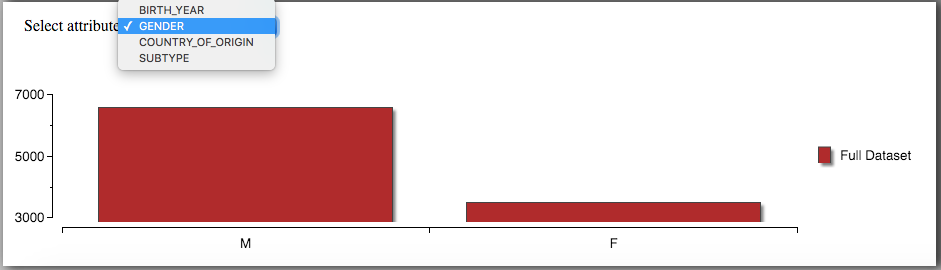
\includegraphics[width=400pt, height=400pt, keepaspectratio=true]{images/change_attr.PNG}
\caption{Change the attribute in the drop down box}
\label{fig:change_attr}
\end{figure}
When you change the attribute by selecting a new value in the drop down box on top of the bar chart (see fig. \ref{fig:change_attr}), the chart will update and now only show data for this specific newly selected attribute.

\subsubsection{View Tree}
\begin{figure}[H]
\centering
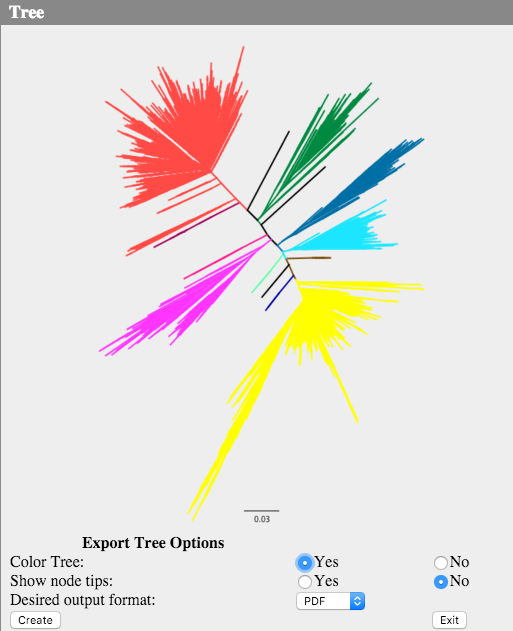
\includegraphics[width=400pt, height=400pt, keepaspectratio=true]{images/view_tree.PNG}
\caption{Tree visualization in FigTree}
\label{fig:view_tree}
\end{figure}
When the 'View Tree' button on top of the circular phylogenetic tree representation is clicked, a popup window will appear such as in fig. \ref{fig:view_tree} where the tree is shown as a radial tree such as it is represented in FigTree. The different clusters get different colours. The colours in the radial tree representation correspond to the colours in the circular tree representation.
\\
In addition to the visualisation of the tree, export options are available. The user can select if he/she wants the tree to be coloured, if the node tips should be shown and in which format the tree will be exported. 

\subsection{PPlacer}
Explanation of the PPlacer here. Not enough relevant data yet. Should be added here.

\end{document}
